\documentclass[12pt,addpoints]{exam}
%\usepackage{enumitem}
\usepackage{amsfonts,amssymb,amsmath, amsthm}
\usepackage{graphicx}
\usepackage{systeme}
\usepackage{pgf,tikz,pgfplots}
\pgfplotsset{compat=1.15}
\usepgfplotslibrary{fillbetween}
\usepackage{mathrsfs}
\usetikzlibrary{arrows}
\usetikzlibrary{calc}
\usepackage{geometry}
\geometry{
	a4paper,
	total={170mm,257mm},
	left=20mm,
	top=20mm,
}
\date{October, 2023}
\pagestyle{headandfoot}
%\firstpageheadrule
\runningheader{Vectors}{}{Page \thepage\ of \numpages}
\runningheadrule
\firstpagefooter{}{}{}
\runningfooter{By Aaron G.K.}{}{Page \thepage\ of \numpages}
\title{Vectors}
\author{Aaron G.K.}
\begin{document}
	\maketitle
	Vectors are essential to physics and engineering. Many fundamental physical quantities are vectors, including displacement, velocity, force, and electric and magnetic vector fields. Scalar products of vectors define other fundamental scalar physical quantities, such as energy. Vector products of vectors define still other fundamental vector physical quantities, such as torque and angular momentum. In other words, vectors are a component part of physics in much the same way as sentences are a component part of literature.
	\subsection*{Scalars and Vectors}
    Many physical quantities can be specified completely by giving a single number and the appropriate unit. For example, “a class period lasts 50 min” or “the gas tank in my car holds 65 L” or “the distance between two posts is 100 m.” A physical quantity that can be specified completely in this manner is called a scalar quantity. Scalar is a synonym of “number.” Time, mass, distance, length, volume, temperature, and energy are examples of scalar quantities.
    \\ \\
    Some other physical quantities, however, cannot be described completely by just a single number of physical units - they may need a direction attached to the scalar to give it the full meaning. Physical quantities specified completely by giving a number of units (magnitude) and a direction are called vector quantities. 
    \subsection*{Representation of Vectors}
    \begin{center}
    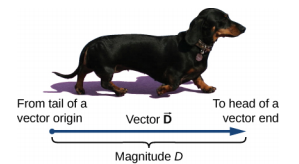
\includegraphics[scale=0.5]{dog.png}	
    \end{center}
    We draw a vector from the initial point or origin (called the \textbf{tail}) to the end or terminal point (called the \textbf{head}), marked by an arrowhead. Magnitude is the length of a vector and is \textbf{always a positive }scalar quantity. \\ \\
    To see how vectors work, let's take a simple displacement vector shown in the figure below.
    \begin{center}
    	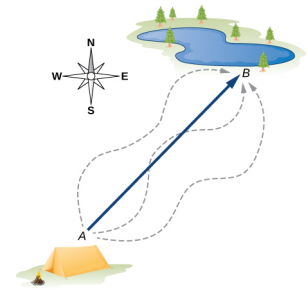
\includegraphics[scale=0.4]{disp.png}
    \end{center}
    The displacement vector from point A to point B is indicated by an arrow with origin at point A and end at point B. The displacement is the same for any of the actual paths (dashed curves) that may be taken between points A and B. \\ \\
    Two vectors that have identical directions are said to be parallel vectors—meaning, they are parallel to each other. Two parallel vectors $\vec{A}$ and $\vec{B}$ are equal, denoted by $\vec{A}=\vec{B}$, if and only if they have equal magnitudes $\vec{A}=\vec{B}$. Two vectors with directions perpendicular to each other are said to be orthogonal/perpendicular vectors. 
    \begin{center}
    	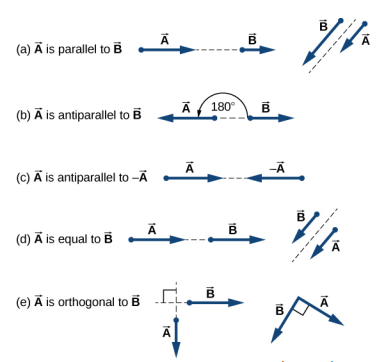
\includegraphics[scale=0.6]{vectors.png}
    \end{center}
    \subsection*{Algebra of Vectors}
    In a vector equation, both sides of the equation are vectors. In general, when a vector $\vec{A}$ is multiplied by a positive scalar $\alpha$, the result is a new vector $\vec{B}$
    that is parallel to $\vec{A}$. The magnitude the new vector($\vec{B}$) is obtained by multiplying the magnitude of the original vector($\vec{A}$) with the scalar.
    $$\vec{B} = \alpha \vec{A}\hspace{1cm}\text{\&}\hspace{1cm}|\vec{B}|= |\alpha| |\vec{A}|$$
    Based on the scalar we multiply the original vector with, we can change the following aspects of the vector
    \begin{itemize}
    	\item if $|\alpha|>1$, the magnitude of the new vector will be larger 
    	\item if $|\alpha|>1$, the magnitude of the new vector will be smaller
    	\item if $\alpha>0$, the new vector will be parallel to the original vector
    	\item if $\alpha<0$, the new vector will be anti-parallel to the original vector
    \end{itemize}
	Most of the applications of vectors lies in operations on vectors. One significant operation is addition of vectors. The sum of vectors is called the resultant. 
	$$\vec{R}=\vec{A}+\vec{B}$$
	For vectors that act along one dimension, it is as simple as adding/subtracting their magnitudes depending on whether they are parallel or anti-parallel. 
	\\ \\
	When adding many vectors in one dimension, it is convenient to use the concept of a unit vector. A unit vector, which is denoted by a letter symbol with a hat, such as  $\hat{v}$, has a magnitude of one and does not have any physical unit. The only role of a unit vector is to specify direction.
	$$\hat{v}=\dfrac{\vec{v}}{|\vec{v}|}$$
	Vector addition has a few of these properties:
	\begin{itemize}
		\item Commutativity $\vec{A} + \vec{B} = \vec{B} + \vec{A}$
		\item Associativity $(\vec{A} + \vec{B}) + \vec{C} = \vec{A} + (\vec{B} + \vec{C})$
		\item Distributive over scalars $\alpha_{1} \vec{A} + \alpha_{2} \vec{A} = (\alpha_{1} + \alpha_{2}) \vec{A}$
	\end{itemize}
	However, when dealing with multi-dimensional(two \& more), we have to have a bit more complicated process to come up at out resultant. One simple way of adding these vectors is using a graphical addition method. The two common ones are the parallelogram method and the more popular, triangle method.
	\subsubsection*{Parallelogram Method}
	Make the parallel translation of each vector to a point where their origins (marked by the dot) coincide and construct a parallelogram with two sides on the vectors and the other two sides (indicated by dashed lines) parallel to the vectors. 
	\begin{center}
		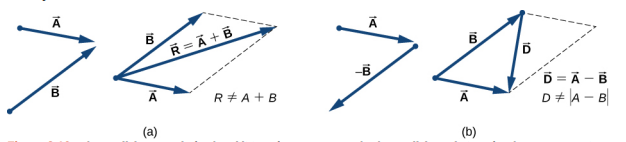
\includegraphics[scale=0.5]{parallelogram.png}
	\end{center}
	\begin{itemize}
		\item $\vec{A}+\vec{B}$ Draw the resultant vector $\vec{R}$ along the diagonal of the parallelogram from the common point to the opposite corner. \textit{\textbf{Length R of the resultant vector is not equal to the sum of the magnitudes of the two vectors}}.
		\item $\vec{A}-\vec{B}$ Draw the difference vector $\vec{D}$ along the diagonal connecting the ends of the vectors. Place the origin of vector $\vec{D}$ at the end of vector $\vec{B}$ and the end of vector $\vec{D}$ at the end of vector $\vec{A}$. \textit{\textbf{Length D of the difference vector is not equal to the difference of magnitudes of the two vectors.}} 
	\end{itemize} 
\end{document}	